\documentclass[11pt,a4paper]{article}

% --- Encoding, language, and margins ---
\usepackage[utf8]{inputenc}
\usepackage[T1]{fontenc}
\usepackage[english]{babel}
\usepackage{geometry}
\geometry{margin=2.5cm}

% --- Math and layout ---
\usepackage{amsmath, amssymb, amsfonts}
\usepackage{graphicx}
\usepackage{float}
\usepackage{fancyhdr}
\usepackage{lastpage}
\usepackage{setspace}
\usepackage{xcolor}
\usepackage{hyperref}
\usepackage{subcaption}
\usepackage{enumitem}
\usepackage[ruled,vlined,linesnumbered]{algorithm2e}
\usepackage{boxedminipage}
\usepackage{amsthm}
\usepackage{tikz}
\usepackage{tikz-cd}

% --- Spacing and style ---
\onehalfspacing
\setlength{\parskip}{0.5em}
\setlength{\parindent}{0pt}

% --- Headers and footers ---
\pagestyle{fancy}
\fancyhf{}
\lhead{\textbf{SF2956: Topological Data Analysis}}
\rhead{Project: Neurons differentiation --- November 2026}
\cfoot{\thepage/\pageref{LastPage}}

% --- Discreet hyperlinks ---
\hypersetup{
    colorlinks = true,
    linkcolor = blue!60!black,
    urlcolor  = blue!70!black
}

% --- Document information ---
\title{Project: Neurons differentiation}
\author{Ahou Lucas\\Powierski Maxim\\Peduzzi Lionel}
\date{November 2026}

\begin{document}

% =========================================================
%                       FRONT PAGE
% =========================================================
\begin{titlepage}
    \thispagestyle{empty}
    \centering
    \vspace*{2cm}

    {\large \textsc{KTH Royal Institute of Technology}\par}
    \vspace{0.5cm}
    {\large SF2956: Topological Data Analysis\par}

    \vspace{2.5cm}
    \hrule height 1pt
    \vspace{0.8cm}
    {\Huge \bfseries Project:\\[0.3em] Neurons differentiation\par}
    \vspace{0.8cm}
    \hrule height 1pt

    \vspace{3cm}
    {\large \textbf{Authors}\par}
    \vspace{0.4cm}
    {\large
    Ahou Lucas\\[0.2em]
    Powierski Maxim\\[0.2em]
    Peduzzi Lionel\par}

    \vfill
    {\large November 2026\par}
    \vspace{1cm}
\end{titlepage}

% =========================================================
%                   TABLE OF CONTENTS
% =========================================================
\pagenumbering{roman}
\setcounter{page}{1}
\tableofcontents
\clearpage

\pagenumbering{arabic}
\setcounter{page}{1}

% =========================================================
%                         CONTENT
% =========================================================
\section{Subject introduction}

Neurons communicate with short electrical pulses called \textbf{spikes}. When we record a neuron, we get a list of the times when it fired. This list is called a \textbf{spike train}. The shape of a single spike carries almost no information: all spikes look the same. The information is in the timing of the spikes.

In the retina, there are many different types of neurons. For example, in the mouse there are more than 30 types of retinal ganglion cells. Each type reacts to a different feature of the image: some react when the light turns on, some when it turns off, some to motion, and so on. Two neurons that see the same image can therefore produce very different spike trains. But two recordings of the same neuron should look similar, even if they are not exactly the same, because neurons are noisy.

This leads to the question of our project:
\begin{center}
    \textit{Given a single spike train, can we tell which neuron it comes from?}
\end{center}
In other words, we want to know if each neuron has its own ``signature'' in its spike trains. If this signature exists, it should also help to separate neurons into groups, and maybe later into cell types.

To study this question, we need a good way to compare spike trains. This is not easy. A spike train is not a vector of fixed size: two trials can have a different number of spikes. Also, small shifts in time should only change the distance a little. Classical tools exist, like comparing histograms of interspike intervals or counting spikes in time windows. In this project, we try to use \textbf{topological data analysis} (TDA) instead. The idea is to transform each spike train into a geometric object, for example a point cloud. Then we use the stable rank (see Section 1) to turn this object into a function. These functions are easy to compare, and the stable rank is stable: a small change in the spike train gives a small change in the function.

To test this, we need data where the same neuron is recorded many times under the same conditions. We use recordings of mouse retinal ganglion cells that see the same white noise movie repeated about 30 times (see Section~3). We then check whether the nearest spike train to a given trial comes from the same neuron. We compare the TDA methods with simpler methods that do not use topology.

\section{Data set}

\subsection{The experiment}
We use a public dataset from Karamanlis and Gollisch\footnote{D. Karamanlis and T. Gollisch (2021), \textit{Nonlinear spatial integration underlies the diversity of retinal ganglion cell responses to natural images}, J Neurosci 41:3479--3498. The data is available on the \href{https://gin.g-node.org/gollischlab/Karamanlis_Gollisch_2021_RGC_spiketrains_natural_image_encoding}{G-Node GIN platform}.}. In this experiment, the retina of a mouse was taken out and placed on a multielectrode array. This array has 252 electrodes. Each electrode records the electrical activity of the neurons that are close to it. The recorded neurons are retinal ganglion cells. These cells are the output neurons of the retina: they send the visual information to the brain.

During the recording, the retina was stimulated with light patterns shown on a small screen. A spike sorting algorithm was then used to find the spikes of each neuron in the electrode signals. The authors also gave a list of the ``good'' neurons, which are the ones that were sorted well. We only use these neurons. The full dataset contains 13 recording sessions.

\subsection{The stimulus}
The authors used many different stimuli. We only use one of them: the \textbf{frozen noise}. It is a white noise movie made of black and white squares. Each square is black or white at random, with probability $1/2$.

The stimulus alternates between two parts:
\begin{itemize}
    \item a \textit{running} part: 1500 frames of new random noise (about 50 seconds),
    \item a \textit{frozen} part: 300 frames of a fixed noise movie (about 10 seconds).
\end{itemize}
The frozen part is always the same movie. So each neuron sees exactly the same stimulus many times. We call each presentation of the frozen part a \textbf{trial}. This is useful for us: since the input is the same, the differences between neurons come from the neurons themselves and not from the stimulus.

\subsection{Building our dataset}
Only 9 of the 13 sessions contain the frozen noise stimulus, so we keep these 9 sessions. For each good neuron, we cut its spike train into trials. A trial starts at the beginning of a frozen part and lasts about 9.94 seconds. We shift the spike times so that each trial starts at time 0. Then we compute the interspike intervals (ISIs), which are the times between two consecutive spikes:
\[
    \text{ISI}_i = t_{i+1} - t_i .
\]
If a trial has less than 2 spikes, its list of ISIs is empty. We keep these trials anyway.

Our final dataset contains:
\begin{itemize}
    \item 850 neurons from 9 sessions,
    \item 30 trials per neuron in most sessions (31 and 34 in two sessions),
    \item 25\,873 spike trains in total (one per neuron and per trial).
\end{itemize}
The neurons fire at very different rates. The median firing rate is 5.7 Hz, and half of the neurons fire between 2.4 Hz and 14.2 Hz. 42 neurons fire less than 0.5 Hz, so they have very few ISIs. We do not have any labels for the cell types. We only know the identity of each neuron.

\subsection{First observations}
Figure~\ref{fig:raster} shows the spikes of one neuron for all its trials. We can see vertical lines: the neuron often fires at the same times in different trials. This means that the response is locked to the stimulus. To check this for all neurons, we computed the correlation between the firing rates of different trials. The median correlation is 0.16. When we shift the trials randomly in time, it drops to 0. So most neurons respond in a reliable way to the frozen noise.

We also noticed that the neurons fire a bit more at the end of the recording than at the beginning (about 93 spikes per trial in the first trials, against about 115 in the last ones). We have to keep this in mind, because the trials are not perfectly identical.

\begin{figure}[H]
    \centering
    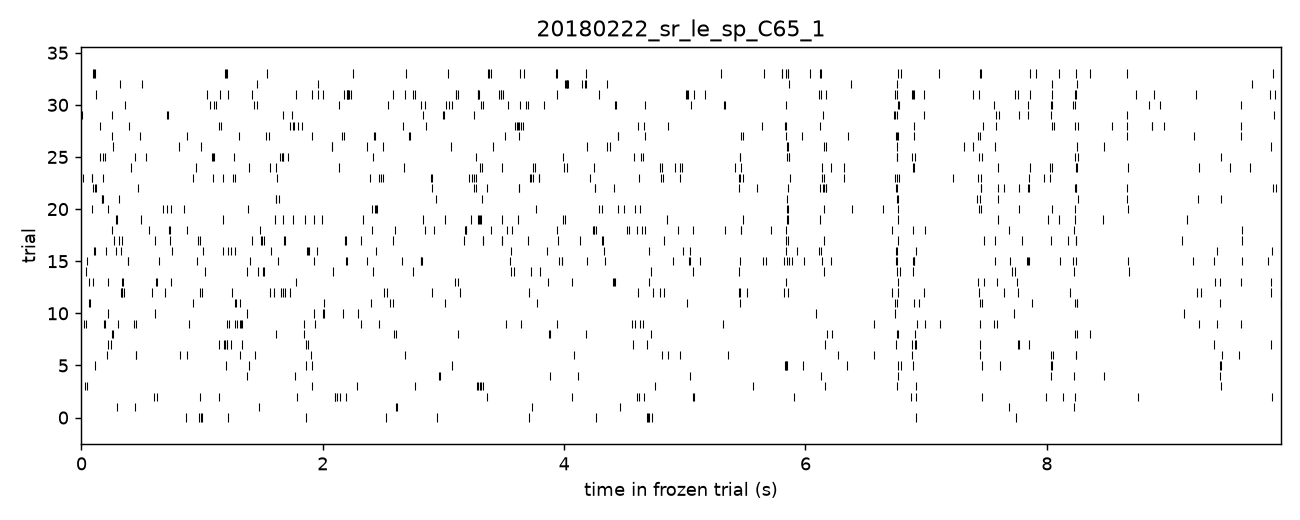
\includegraphics[width=0.95\linewidth]{raster_20180222_sr_le_sp_C65_1.png}
    \caption{Raster plot of one neuron (session 20180222\_sr\_le\_sp). Each line is one trial, and each tick is a spike.}
    \label{fig:raster}
\end{figure}








\section{Mathematical background}
Before using any methods to analyse the dataset, we will introduce the main ideas of the methods and the mathematical concepts needed to understand these methods.

\subsection{Framework}
The basic idea of the method is to transform any dataset into a mathematical object on which it is more convenient to perform statistical and ML analysis. More formally, our data sets are described by a metric space $(X,d)$ and we would like to map it to a piecewise constant function. This procedure tries to capture the stucture/invariant of this dataset.

Here are two ways to describe the procedure of the method:

\textbf{First:}
\begin{enumerate}
    \item Choose an extension $\psi$ and create a dendrogram $D$ as the hierarchical clustering of $X$ with respect to $\psi$
    \item Choose a field K and create tame vector space parametrized by $[0,\infty)$: $V=KD$
    \item Use the stable rank to transform the vector space into a PCF.
\end{enumerate}

\textbf{Second:}
\begin{enumerate}
    \item Create a simplicial complex from X through Vietoris-Rips: $S=VR_t(X)$
    \item Choose a field K and create the $n^{th}$ homology of $S$: $V=H_n(S,K)$
    \item Use the stable rank to get a PCF: $\widehat{rank}\,V(t)$
\end{enumerate}

The first procedure with a single linkage as an extension is equivalent to the second one with $n=0$. But, by increasing $n$, we can get a new family of methods that provide more information about the data set.


\subsection{Hierarchical clustering}
Clustering consists in grouping the points of a dataset $(X,d)$ so that points in the same group are close to each other.
 
Hierarchical clustering returns a family of nested partitions, from the finest one (every point alone) to the coarsest one (a single cluster). 

To merge clusters, we need a notion of distance between clusters, not only between points.
 
\textbf{Definition:}
An \emph{extension} (or \emph{linkage}) $\psi$ transforms a distance $d$ between elements of $X$ into a distance $\psi d$ between non-empty subsets $A,B \subseteq X$, such that $\psi d(\{x\},\{y\}) = d(x,y)$ for all $x,y\in X$.
 
Here are two examples of extensions.
\begin{align*}
\psi_{\text{single}}(A,B) &= \min_{a\in A,\, b\in B} d(a,b), &
\psi_{\text{complete}}(A,B) &= \max_{a\in A,\, b\in B} d(a,b)
\end{align*}
 
\textbf{Algorithm:}
Given $(X,d)$ and an extension $\psi$:
\begin{enumerate}
    \item Start with the partition $P_0=\{\{x\} \mid x\in X\}$ and set $a_0=0$.
    \item For $k=0,\dots,N-2$: choose two distinct elements $A,B$ of $P_k$ that minimise $\psi d(A,B)$, set $a_{k+1}=\psi d(A,B)$ and
    \[
        P_{k+1} = \big(P_k \setminus \{A,B\}\big)\cup\{A\cup B\}.
    \]
\end{enumerate}
The output is the sequence of partitions $P_0, P_1, \dots, P_{N-1}=\{X\}$ and the sequence $a_0,\dots,a_{N-1}$.

Remark: If there exist several pairs $A,B$ of $P_k$ that minimise $\psi d(A,B)$, we can merge them at the same time to make the transformation independent of the order of the elements.

 
\subsection{Dendrograms}
The output of the hierarchical clustering is encoded by an object called a dendrogram.
 
\textbf{Definition:}
A \textbf{dendrogram} of $X$ is defined by associating to each value of $t \in [0,\infty)$ a partition $D_t$ of $X$. It must also contain the definition of the maps between partitions: $\forall t_1, t_2 \in [0,\infty) \, s.t. \, t_1<t_2: \exists D_{t_1<t_2}: D_{t_1} \rightarrow D_{t_2}$. And the following properties must be fulfilled:

$\forall t_1, t_2, t_3 \in [0,\infty) \, s.t. \, t_1<t_2<t_3:  D_{t_2<t_3} (D_{t_1<t_2}) = D_{t_1<t_3}$.

There must also exist a sequence of real numbers: $0=a_0<a_1<\dots<a_n$ such that the transition between $D_{t_1}$ and $D_{t_2}$ is an isomorphism if $t_1$ and $t_2$ belong to the same interval among $[a_0,a_1),[a_1,a_2),\dots,[a_n,\infty)$.
 
\textbf{Dendrogram as a graph:}
It can be represented by a graph where lines gather when the set merges. 
 
\begin{figure}[H]
    \centering
    \begin{tikzpicture}[x=1.1cm, y=0.75cm]
        % leaves a,b,c,d,e at x = 0,...,4 ; merge heights 1, 1.5, 2, 3.5
        \draw[->] (-0.8,0) -- (-0.8,4.6) node[above] {$t$};
        \foreach \h in {0,1,2,3,4} \draw (-0.85,\h) -- (-0.75,\h) node[left=2pt, font=\small] at (-0.85,\h) {\h};
        % merge a-b at 1
        \draw (0,0) -- (0,1) -- (1,1) -- (1,0);
        % merge (ab)-c at 1.5
        \draw (0.5,1) -- (0.5,1.5) -- (2,1.5) -- (2,0);
        % merge d-e at 2
        \draw (3,0) -- (3,2) -- (4,2) -- (4,0);
        % final merge at 3.5
        \draw (1.25,1.5) -- (1.25,3.5) -- (3.5,3.5) -- (3.5,2);
        \foreach \x/\l in {0/a,1/b,2/c,3/d,4/e} \node[below] at (\x,0) {$\l$};
    \end{tikzpicture}
    \caption{Example of a dendrogram of five elements set.}
    \label{fig:dendrogram}
\end{figure}

When we have the dendrogram we can transform it into a parametrized tame vector space and then we compute its stable rank (more information on this in the next sections).
 

\subsection{Simplicial complexes}
The first step of partitioning $X$ makes us lose information about the dataset (if it is not an ultra pseudo-metric). This is what motivates the use of simplicial complexes. A simplicial complex is the generalisation of a graph, it contains nodes, edges, and higher dimensional objects like triangles, tetrahedra, etc. 

\textbf{Definition:}
Let the set $\mathcal{U}$ be called a universe.
A simplicial complex is a set of simplices of different orders. A simplex of dimension $n$ is a set of $n+1$ elements of $\mathcal{U}$. And a simplicial complex $S$ must contain every non-empty subset of its simplices (If $\sigma \in S \Rightarrow$ all non-empty subset of $\sigma \in S$). 

We can create a simplicial complex from a metric space by using Vietoris-Rips. This tool allows to lose no information on $(X,d)$. 

\textbf{Definition:}
$VR_t(X)$ is the collection of non-empty subset $\sigma$ of $X$ such that $\forall x,y \in \sigma, d(x,y)\leq t$.


\subsection{Tame vector space parametrized by $[0,\infty)$}
Tame vector space parametrized by $[0,\infty)$ is defined by choosing for each value of $t \in [0,\infty)$ a finite dimensional vector space. It must also contain the definition of the maps between these vector spaces: $\forall t_1, t_2 \in [0,\infty) \, s.t. \, t_1<t_2: \exists V_{t_1<t_2}: V_{t_1} \rightarrow V_{t_2}$.

And we must verify the following properties:

$\forall t_1, t_2, t_3 \in [0,\infty) \, s.t. \, t_1<t_2<t_3:  V_{t_2<t_3} (V_{t_1<t_2}) = V_{t_1<t_3}$.

There must exist a sequence of real numbers: $0=a_0<a_1<\dots<a_n$ such that the transition between $V_{t_1}$ and $V_{t_2}$ is an isomorphism if $t_1$ and $t_2$ belong to the same interval among $[a_0,a_1),[a_1,a_2),\dots,[a_n,\infty)$.




\subsection{Homology}
This step allows us to transform a simplicial complex into a tame-vector space while keeping the invariants. Here, the invariants that are kept are the ones based on homology.

For a simplicial complex $S$, $S_n$ contains all the simplices of dimension $n$.

We need to choose an ordering of the vertices and then let $d_i:S_n \rightarrow S_{n-1}$ be the map that removes the $i^{th}$ vertex.

We need to choose a field $K$ to create the functions $Kd_i: K^{|S_n|} \rightarrow K^{|S_{n-1}|}$

Let the \textbf{Boundary function} be $\delta_{n}(\sigma) \longmapsto \sum_{i=0}^{n}(-1)^i Kd_i \sigma: K^{|S_n|} \rightarrow K^{|S_{n-1}|}$

We can observe that $\ker(\delta_{n})$ represents the cycles of order $n$ and that $\text{im}(\delta_{n+1})$ represent the boundaries of order $n$. As $\text{im}(\delta_{n+1}) \subseteq \ker(\delta_{n})$ we can construct the $n^{th}$ homology as 

\textbf{Definition:}
$H_n(S, K) := \ker(\delta_n)/\text{im}(\delta_{n+1})$

Intuition:

When n=0, $\ker(\delta_0)$ contains all the vertices of order 0. $\text{im}(\delta_{1})$ makes all the vertices connected by an edge equivalent. Then, all the vertices in the same connected component are equivalent and the number of elements is equal to the number of connected components.

When n=1, $\ker(\delta_1)$ contains all the loops (a sequence of edges that starts and ends at the same vertex). $\text{im}(\delta_2)$ contains the loops that encircle an order 2 vertex. We end up with only the loops that don't encircle an order 2 vertex.

\begin{figure}[H]
    \centering
    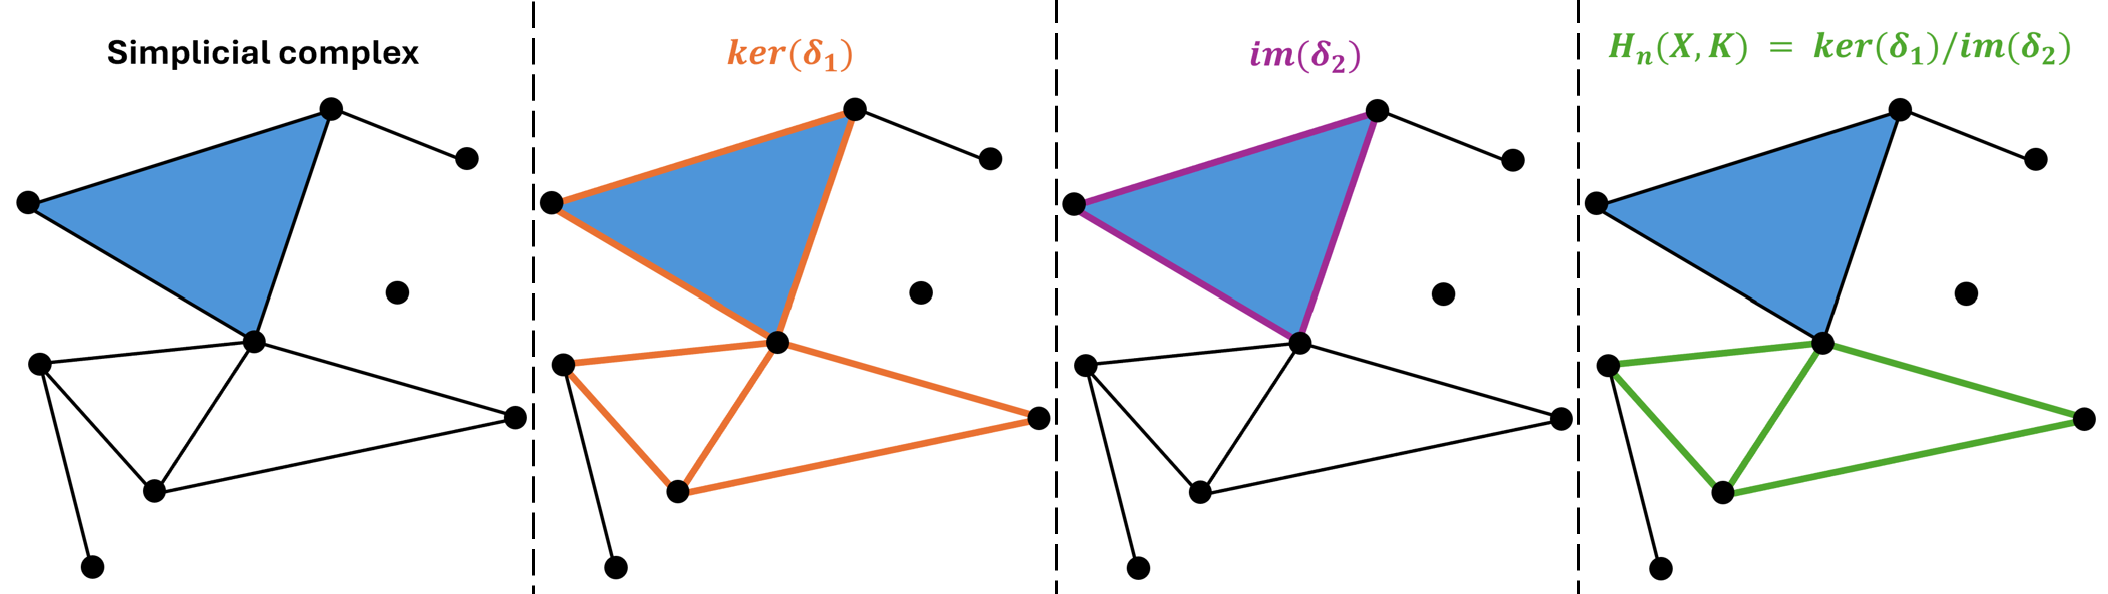
\includegraphics[width=0.99\linewidth]{report/2nd_homology.png}
    \caption{Example of $2^{nd}$ homology}
    \label{fig:placeholder}
\end{figure}

\subsection{Stable rank}
The final step is to transform the parametrized tame vector space (PTVS) into a PCF. A straightforward solution would be to take the rank of the vector space, but this is not stable. To address this, we define the \textbf{stable rank}.

To have a stable map, we need one for which the output doesn't vary too much when the input is slightly modified. First, we need an idea of distance between PTVS to measure how much one varies under a change. Let $V$, $W$ be PTVS,

$d_{\bowtie}(V,W) := \inf \left\{ \epsilon + \tau | V \xrightarrow\psi U \xleftarrow\phi W, \psi \text{ is }\epsilon\text{-eq.}, \phi \text{ is }\tau\text{-eq.} \right\}$

where $V \xrightarrow\psi U$ is an $\epsilon\text{-eq.}$ if $\forall t$,  there is a dotted linear function making the
following diagram commutative:

\[
\begin{tikzcd}[column sep=3cm, row sep=1.5cm]
V_t
    \arrow[r, "V_{t<t+\epsilon}"]
    \arrow[d, "\psi_t"']
&
V_{t+\epsilon}
    \arrow[d, "\psi_{t+\epsilon}"]
\\
W_t
    \arrow[r, "W_{t<t+\epsilon}"']
    \arrow[ur, dotted]
&
W_{t+\epsilon}
\end{tikzcd}
\]

This distance is a metric and we can now define the stable rank as:

\textbf{Definition:}
$\widehat{rank}\,V(t) := \min\left\{ rank(W) | d_{\bowtie}(V,W)\leq t \right\}$





\section{Methods}
% TODO: 
\subsection{Embeddings}
In order to use the topological data analysis pipeline, we will transform each spike train into a point cloud. There is no straightforward way to achieve this, so we will present different possibilities.

\subsubsection{Distance-based}

\subsubsection{Time-based}

\subsubsection{Cross-correlation}

\subsubsection{Spectral/Frequency}

\subsubsection{Probabilistic}




\section{Results}
% TODO: persistence diagrams, comparisons, interpretation.

\end{document}